\documentclass[11pt]{article}\usepackage[]{graphicx}\usepackage[]{color}
% maxwidth is the original width if it is less than linewidth
% otherwise use linewidth (to make sure the graphics do not exceed the margin)
\makeatletter
\def\maxwidth{ %
  \ifdim\Gin@nat@width>\linewidth
    \linewidth
  \else
    \Gin@nat@width
  \fi
}
\makeatother

\definecolor{fgcolor}{rgb}{0.345, 0.345, 0.345}
\newcommand{\hlnum}[1]{\textcolor[rgb]{0.686,0.059,0.569}{#1}}%
\newcommand{\hlstr}[1]{\textcolor[rgb]{0.192,0.494,0.8}{#1}}%
\newcommand{\hlcom}[1]{\textcolor[rgb]{0.678,0.584,0.686}{\textit{#1}}}%
\newcommand{\hlopt}[1]{\textcolor[rgb]{0,0,0}{#1}}%
\newcommand{\hlstd}[1]{\textcolor[rgb]{0.345,0.345,0.345}{#1}}%
\newcommand{\hlkwa}[1]{\textcolor[rgb]{0.161,0.373,0.58}{\textbf{#1}}}%
\newcommand{\hlkwb}[1]{\textcolor[rgb]{0.69,0.353,0.396}{#1}}%
\newcommand{\hlkwc}[1]{\textcolor[rgb]{0.333,0.667,0.333}{#1}}%
\newcommand{\hlkwd}[1]{\textcolor[rgb]{0.737,0.353,0.396}{\textbf{#1}}}%
\let\hlipl\hlkwb

\usepackage{framed}
\makeatletter
\newenvironment{kframe}{%
 \def\at@end@of@kframe{}%
 \ifinner\ifhmode%
  \def\at@end@of@kframe{\end{minipage}}%
  \begin{minipage}{\columnwidth}%
 \fi\fi%
 \def\FrameCommand##1{\hskip\@totalleftmargin \hskip-\fboxsep
 \colorbox{shadecolor}{##1}\hskip-\fboxsep
     % There is no \\@totalrightmargin, so:
     \hskip-\linewidth \hskip-\@totalleftmargin \hskip\columnwidth}%
 \MakeFramed {\advance\hsize-\width
   \@totalleftmargin\z@ \linewidth\hsize
   \@setminipage}}%
 {\par\unskip\endMakeFramed%
 \at@end@of@kframe}
\makeatother

\definecolor{shadecolor}{rgb}{.97, .97, .97}
\definecolor{messagecolor}{rgb}{0, 0, 0}
\definecolor{warningcolor}{rgb}{1, 0, 1}
\definecolor{errorcolor}{rgb}{1, 0, 0}
\newenvironment{knitrout}{}{} % an empty environment to be redefined in TeX

\usepackage{alltt}

\usepackage{rotating}
\usepackage{graphics}
\usepackage{latexsym}
\usepackage{color}
\usepackage{listings}
\usepackage{wrapfig}
\usepackage{float}
\usepackage[belowskip=-15pt,aboveskip=0pt]{caption}

\setlength\topmargin{-.56in}
\setlength\evensidemargin{0in}
\setlength\oddsidemargin{0in}
\setlength\textwidth{6.49in}
\setlength\textheight{8.6in}
\setlength{\intextsep}{10pt plus 1pt minus 4pt}

\definecolor{codegreen}{rgb}{0,0.6,0}
\definecolor{codegray}{rgb}{0.5,0.5,0.5}
\definecolor{codepurple}{rgb}{0.58,0,0.82}
\definecolor{backcolour}{rgb}{0.95,0.95,0.92}
\lstdefinestyle{mystyle}{
	backgroundcolor=\color{backcolour},   
	commentstyle=\color{codegreen},
	keywordstyle=\color{magenta},
	numberstyle=\tiny\color{codegray},
	stringstyle=\color{codepurple},
	basicstyle=\footnotesize,
	breakatwhitespace=false,         
	breaklines=true,                 
	captionpos=b,                    
	keepspaces=true,                 
	numbers=left,                    
	numbersep=5pt,                  
	showspaces=false,                
	showstringspaces=false,
	showtabs=false,                  
	tabsize=2
}
\lstset{style=mystyle}

\pagestyle{headings}

\title{Statistical Analysis and Predictive Models for Expenditures in New York Municipalities\vspace{-5ex}} 
\date{October 08, 2020\vspace{-5ex}}
\IfFileExists{upquote.sty}{\usepackage{upquote}}{}
\begin{document} 
\maketitle
\hfill \break








\noindent\textbf{Executive Summary} 

\noindent In New York, there are many new housing projects started daily. Given the issue that the town need to generate more funding through property tax when expenditures increases. However, there is no clear understanding of which factors cause the expenses to increase/decrease. Therefore, a clear goal for this analysis is to find variables that effect expenditures in New York. A tool was developed using multiple linear regression models to predict expenditures using a dataset from the New York municipalities from 1992. With an adjusted R-square of 61\%, a final model was chosen after stepwise variables selection process with AIC, MSE, and adjusted R-square criteria. The variables in the final model includes population, wealth, income, percent intergovernmental funds, and growth rate. Diagnostics measurements was also built to check for the quality of the model. Some interesting findings include a 4\% increase in expenditures while wealth increases by 10\%. On the other hand, there will be a 3\% decrease in expenditures while the percentage of intergovernmental funds increases by 10\%. Knowing the changes in expenditures caused by wealth, population, intergovernmental funds, and growth rate, construction workers and properties owners would be more caution when starting a new project.            
\hfill \break

\noindent\textbf{Introduction} 

\noindent Generally, construction companies have numerous aspects in estimating the cost of each new housing project. To estimate the cost of each housing project, expenditures play an important role in increasing or decreasing the cost. For example, higher expenditures would result in an increase in cost of construction. Therefore, the property owners would have to seek for higher funding to fulfill the project. On the other hand, while expenditures decrease, property’s owners could reimburse the expenses elsewhere. In addition, knowing the expenditures would also help construction managers to order supplies in a proper manger. If expenditures decrease, then the supplies would have to be less in quantity or cheaper in quality. Numerous questions were proposed in favor of these issues such as 1) What variables cause the fluctuation of expenditure? 2) What is the best predictive model that could predict expenditures? 3) How can we validate and implement the model? 3) How accurate is the model? 4) Is there any improvement to the future models? To answer these questions, this analysis will take a deep dive into the data exploratory analysis, model development process using multiple linear regression, and diagnostics analysis. With the answered questions, construction workers and property owners would have a better understanding of their expenditures when starting a new project to avoid over or underestimating their budgets.
\hfill \break

\noindent\textbf{Methods} 

\noindent A dataset from New York municipalities were provided to access the important measures to predict expenditures. These data contain a total of 916 observations from 1992 with 2 observations contain missing expenditures values. Two observations with NA expenditures have been removed from the analysis to improve the assumption of linear regression model. In terms of variables, this dataset contains three identifiers including identity number, state code, and county code, and six demographic and income-related variables including wealth per person, population, percent intergovernmental funding, density, mean income per person, and growth rate. There is a total of 57 distinct county code implying that there are multiple measurement of expenditures per county in New York. The goal of this data analysis is to predict expenditures of two New York municipalities, Warwick and Monroe. A projection dataset for Warwick and Monroe town was also provided to generate predictions using the fitted model. To achieve this goal, all analysis will be done using multiple linear regressions for model development process and accompany by diagnostics process to check for the quality of the model. All analysis including coding and writing report was done in R Studio with R version 3.6.2.     
\hfill \break

\noindent\textbf{Exploratory Data Analysis} 

\noindent During the exploratory analysis process, it is important to access all the significant relationship of each variable with the target variable. Initially, looking at Table~\ref{descrips}, the summary statistics of all independent variables and target variable shows the maximum for expenditures, wealth, population, pint, density, income, and growth rate are extremely high compare to their mean and 75 percentiles. This indicates that all the variables mentioned previously are heavily right skewed. Most importantly, expenditures’ skewness violates the normality assumption when generating a linear regression. Therefore, a log-transformation was applied to expenditures to normalize the distribution of the target variable. Log-transformation would reduce the values which would account for outliers. Figure~\ref{inital-explore}.1 depicts the normality of the outcome variable expenditures after transformation implying the assumption is not violated anymore.

\begin{figure}[h!] 
\begin{center}

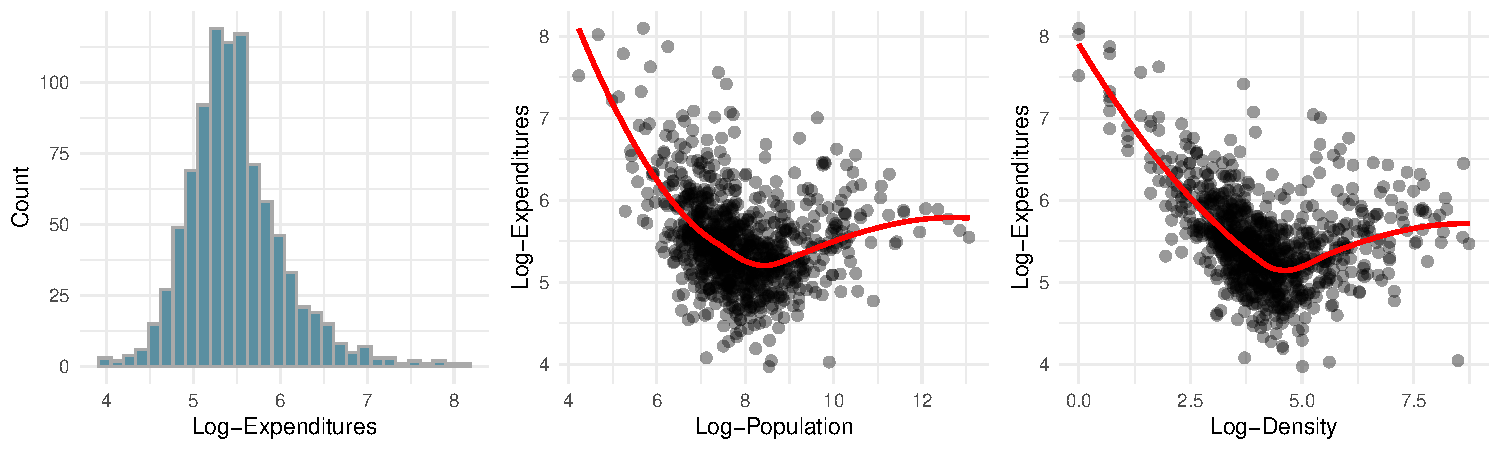
\includegraphics[width=\maxwidth]{figure/unnamed-chunk-1-1} 

\caption{Initial Exploratory plots after log-transformation of 1: Histogram of Log-Expenditures with frequency, 2: Scatter plot of Log-Expenditures vs Log-Population with LOESS smooth line in red, and 3: Scatterplot of Log-Expenditures vs Log-Density with LOESS smooth line in red.}
\label{inital-explore}
\end{center} 
\end{figure}

\noindent Since all independent variables are right-skewed, a log-transformation also applied to each variable to ensure linear relationship with expenditures. An amount of 1.01 was added to all growth rate values to account for zeros values while taking logarithm. All variables mentioned in the rest of this article are log-transformed variables unless otherwise specified. With that being said, wealth, percent intergovernmental funds, income, and grow rate seems to have linear relationship with expenditures. However, population and density have two difference trends of expenditures within their plots. Figure~\ref{inital-explore}.2 shows a scatterplot of expenditures and population with a dip at approximately 8.3 to change direction of correlation. Population is self-explanatory variable which represent the number of people living in the county during the year. While population is less than 8.3, as population increases, expenditures decrease on average. When population is greater than 8.3, expenditures increase as population increases. Similar issue happens to density at 4.5, see Figure~\ref{inital-explore}.3 Density, here, represents the population of other substances like animals, environment, or other objects. To account for this problem, the data set of New York city will be subsetted into different groups according to each trend. Subsetting data will help the relationship between density and population and expenditures be linear. This analysis will only model data when population is greater than 8.3 and density is greater than 4.5 since the projection data is within these ranges.    
\hfill \break



\noindent After selecting a subset of data, only 228 observations are left in the data. A second round of data exploratory was conducted to ensure the relationship of each measure if significant to the outcome variable expenditures. Expenditures and wealth have a positive relationship indicating the increases of wealth would cause expenditure to be higher, see Figure~\ref{sec-explore}.1 Intuitively, this makes sense since wealthier individuals would spend more resulting in higher expenses. Similarly, Figure~\ref{sec-explore}.2 shows a strong positive correlation between expenditure and income. This relationship is expected since the mean income per person is higher, their expenses would also be higher compared to lower income individuals. Other variables like population and density seem to have moderate positive relationship with expenditures, see the first two plots in Figure~A\ref{sec2-explore}. Clearly, population and density are important measurements to predict expenditures. As population and density increases, the amount of expenses also increases, on average. On the other hand, predictors including percent intergovernmental funds and growth rate have moderate negative correlation with expenditures. This indicates that, while percent intergovernmental funds and growth rate increases, the amount of expenses should decrease. This makes perfect sense since if the growth rate in economic is slow, then there would be lower expenses.             

\begin{figure}[h!] 
\begin{center}

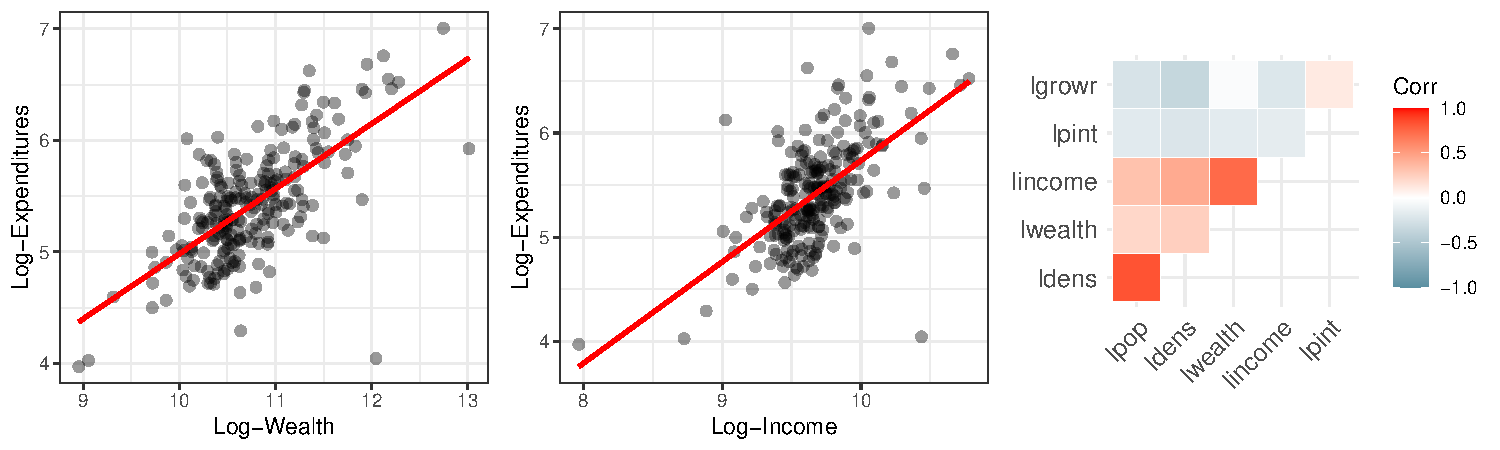
\includegraphics[width=\maxwidth]{figure/unnamed-chunk-3-1} 

\caption{Exploratory plot after log-transformation and subsetted data 1: Scatterplot of Log-Expenditures vs Log-Wealth with Linear Regression line in red, 2: Scatterplot of Log-Expenditures vs Log-Income with linear regression line in red, and 3: Upper Correlation plot of all independent variables.}
\label{sec-explore}
\end{center} 
\end{figure}

\noindent After detecting the relationship of each independent variables with expenditures, it is important to examine the correlation of each predictors. Higher correlation between predictors mean there might be multicollinearity issues when including both variables in the model. This leads the model to have unstable and unreliable coefficients. Figure~\ref{sec-explore}.3 shows the upper diagonal of the correlation matrix plot. As one can see, density and population have a high positive correlation of 0.83. To solve the multicollinearity issues, separate models with density in one and population in other, along with other variables, were generated. The results of the models will be compared and selected as the best model. Furthermore, wealth and income also have high positive correlation of 0.74. However, wealth and income are not strongly correlated. Other variables did not mentioned above have little to no relationship with expenditures.          
\hfill \break

\noindent\textbf{Statistical Analysis}



\noindent Model selection is a crucial step in a data analysis. Multiple linear regressions will be used to build all the models. After the exploratory data analysis, there are six possible variables that can be include in the model including wealth, population, percent intergovernmental funds, density, income, and growth rate. As mentioned before, if population and density are in the same models, multicollinearity issues will occur. Therefore, two initial models will be built to compared using three validation metrics such as Akaike information criterion (AIC), R-squared adjusted, and mean square error (MSE). In this case, the ideal best model would have smaller AIC score, higher R-square adjusted, and lower MSE. After building both models, a table of model comparison was generated to select the best model among the two, see Table~B\ref{reg_vali_metric}. This table clearly states that the second model with predictors wealth, population, percent intergovernmental funds, income, and grow is the best model with lower MSE and AIC values, and higher R-square adjusted with the values of 0.09, 124.16, and 0.61, respectively.

\noindent After finding the best predictors for the model (wealth, population, percent intergovernmental, income, and growth rate), a stepwise selection method was generated for variables selection using AIC values. Unfortunately, stepwise variable selection was not showing any other significant models beside the full model. Furthermore, each combination of the interaction predictors was also taken into consideration to find a better model. Results of MSE, R-square adjusted, and AIC for the model with interaction terms (model 3 in Table~B\ref{reg_vali_metric}) are clearly better than model 2. Thus, a stepwise selection method was applied to select the best variables using interaction terms and results are shown in Table~B\ref{reg_vali_metric}) as model 4. Model 4 has the best adjusted R-squared due to the higher number of variables contain in the model. However, in terms of the model's quality, model 4 seems to have insignificant predictors including wealth and wealth times population, see p-value column in Table~B\ref{reg_summary_4}). In addition, the coefficient for percent intergovernmental funds was expected to be negative as shown in Figure~A\ref{sec2-explore}). These two reasons prove that model 4 with interaction terms is not the best model. Therefore, the model with predictors wealth, population, intergovernmental funds, income, and growth rate will be used as the final model.

\noindent After variable selection, diagnostics process is a must to check for the quality of the model. Figure~\ref{diag-plot1}.1 shows the studentized residuals and majority are within the range of -2.5 to 2.5 except one observation 893. This indicates that is observation is an outlier. In addition, Figure~\ref{diag-plot1}.2 shows the cook's distance of all the observations and found that there are a few observations did not make the cutoff point for influential values including index 60, 83, 100, 179, and 225. As seen in Table~A\ref{outlier_obs}, outliers and influential points have high values of either expenditures or one of the predictors. However, none of the outliers and influential points were removed because there are no good reasons. Last but not least, the right plot in Figure~\ref{diag-plot1}.3 shows that studentized residuals follow a normal distribution implying the error terms are constant.    

\begin{figure}[h!] 
\begin{center}

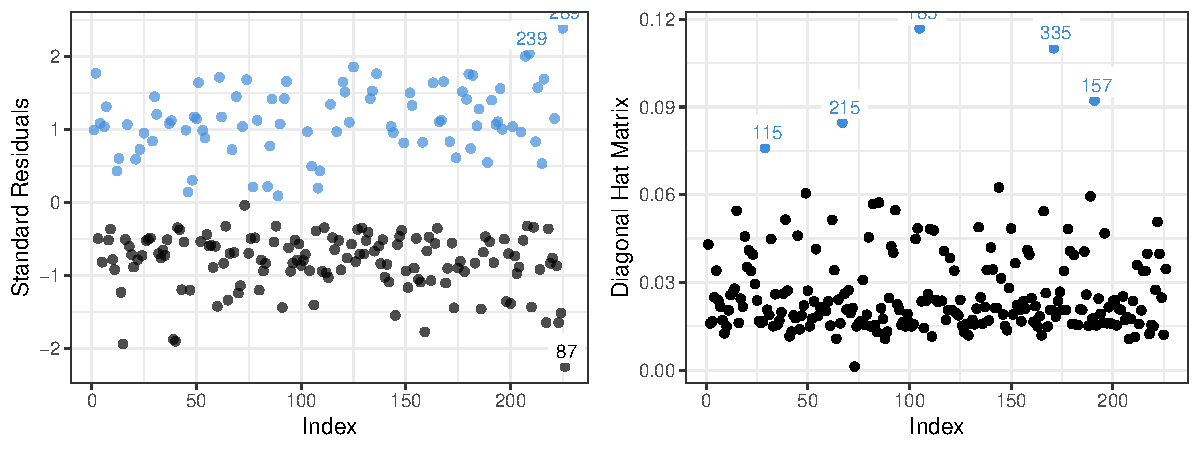
\includegraphics[width=\maxwidth]{figure/unnamed-chunk-5-1} 

\caption{Diagnostic plots of 1: Studentized Residuals vs Predicted values, 2: Cook's distance for each observation, and 3: Distribution of studentized residuals.}
\label{diag-plot1}
\end{center} 
\end{figure}

\noindent After accessing the quality of the model, an interpretation and explanation of the model will be explained. The summary of regression for the final model (wealth, population, intergovernmental, income, and growth rate) is in Table~\ref{reg_summary_final}. VIF values are all smaller than 3 indicating there is no multicollinearity problem in the model. Confident intervals for majority of coefficients do not contain zeros and small p-values implying they are statistically significant in the model. For the purpose of interpreting the model, the coefficient will be back transformation. This means that as wealth, population, or income increases by 10\%, holding all else constant, expenditures will increase by 4\%, 1\%, or 2\%, on average, respectively. On the other hand, while percent intergovernmental fund or growth rate increases by 10\%, on average, expenditures will decrease by 3\% or 1\%, respectively. In addition, this model has an adjusted R-square of 0.61 indicating that 61\% of the variation in expenditure can be explained by wealth, population, percent intergovernmental funds, income, and growth rate.   

\begin{center}
% latex table generated in R 3.6.2 by xtable 1.8-4 package
% Thu Oct 08 15:23:51 2020
\begin{table}[ht]
\centering
\begin{tabular}{lrrrrrrrr}
  \hline
term & estimate & std.error & statistic & p.value & 10\% Coef & 2.5 \% & 97.5 \% & VIF \\ 
  \hline
(Intercept) & -1.2222 & 0.7048 & -1.7340 & 0.0843 & 0.8900 & -2.6112 & 0.1669 &  \\ 
  lwealth & 0.4158 & 0.0553 & 7.5171 & 0.0000 & 1.0404 & 0.3068 & 0.5248 & 2.3499 \\ 
  lpop & 0.0790 & 0.0248 & 3.1873 & 0.0016 & 1.0076 & 0.0302 & 0.1279 & 1.1791 \\ 
  lpint & -0.3077 & 0.0432 & -7.1254 & 0.0000 & 0.9711 & -0.3928 & -0.2226 & 1.0623 \\ 
  lincome & 0.2294 & 0.1052 & 2.1795 & 0.0303 & 1.0221 & 0.0220 & 0.4367 & 2.5248 \\ 
  lgrowr & -0.0198 & 0.0119 & -1.6679 & 0.0968 & 0.9981 & -0.0432 & 0.0036 & 1.1281 \\ 
   \hline
\end{tabular}
\caption{Summary Regression of final model} 
\label{reg_summary_final}
\end{table}

\end{center}

\noindent Given a good model, the goal of this analysis is to predict expenditures for two New York municipalities Warwick and Monroe. A projection table of values was provided to predict from years 1992, 2005, and 2025. Table~\ref{pred_tab} shows a prediction table of the two towns. The values for expenditures seem to be within the range of expenditures in the training set. Looking closely at the projection table, predicted expenditures are higher, on average, in Monroe than Warwick due to the extremely lower percentage of intergovernmental funds and relatively lower growth rate. According to the model, having lower intergovernmental funds and growth rate leads to higher expenditures. Although, Warwick town has relatively higher population, wealth, and income, on average, Monroe town would still have higher expenditures. The last two columns depict lower and upper 95\% confident interval of predicted values and we can say that expenditures are confident to be inside these ranges. Given the coefficients being fixed, Warwick and Monroe would expect their expenditures to change if their wealth, population, percent intergovernmental, income, and growth rate change.    

\begin{center}
% latex table generated in R 3.6.2 by xtable 1.8-4 package
% Thu Oct 08 15:23:51 2020
\begin{table}[ht]
\centering
\begin{tabular}{lrrrrrrrrr}
  \hline
town & year & pop & wealth & pint & income & growr & expen\_hat & expen\_lci & expen\_uci \\ 
  \hline
Warwick & 1992.0 & 16225.0 & 72908.0 & 24.7 & 19044.0 & 30.3 & 233.3 & 125.1 & 435.0 \\ 
  Warwick & 2005.0 & 20442.0 & 85000.0 & 24.7 & 19500.0 & 35.0 & 254.0 & 136.0 & 474.2 \\ 
  Warwick & 2025.0 & 31033.0 & 89000.0 & 26.0 & 20000.0 & 40.0 & 264.2 & 141.1 & 494.5 \\ 
  Monroe & 1992.0 & 9338.0 & 55067.0 & 8.8 & 16726.0 & 30.0 & 265.1 & 142.7 & 492.3 \\ 
  Monroe & 2005.0 & 10496.0 & 58000.0 & 8.8 & 17100.0 & 35.0 & 274.0 & 147.5 & 508.9 \\ 
  Monroe & 2025.0 & 13913.0 & 60000.0 & 10.1 & 18000.0 & 35.0 & 275.5 & 148.3 & 511.8 \\ 
   \hline
\end{tabular}
\caption{Prediction table of two municipalities in New York (Warwick and Monroe)} 
\label{pred_tab}
\end{table}

\end{center}

\noindent\textbf{Conclusion}

\noindent In conclusion, expenditures are one of the most important aspects to know before starting a new construction project. It is difficult to estimate expenditures manually. Therefore, this analysis creates a tool to automate the process of estimating expenditures. The variables that cause the fluctuation of expenditures are population, wealth, percent intergovernmental funds, income, and growth rate. With this model, construction managers and property owners would have a clear understanding of how much funding they would need for a certain type of project in the city. Using the summary regression results of our model, it is confident to say that an area with higher population would cause expenditures to be higher. Similarly, if the average of wealth and income is higher, then expenditures will also be higher. However, it is clear that if the percentage of intergovernmental funds is lower and growth rate in the city is slower, then expenditures is obviously higher. As a result, this model does not only provide an estimate of expenditures faster, but construction workers can also have a great understanding of what cause the expenses to shift up and down.

\noindent There are a few limitations in this analysis. This model only uses a subset of the main data which is 0.2 times less compared to the full dataset. Therefore, smaller sample size would lead the model to perform not as accurate. Second, growth rate has a small correlation with expenditures indicating the amount the changes in expenditures would be very small if the values of growth rate change. Last but not least, the model is only limited to when population is greater than 4024. Cities with population smaller than 4024 cannot use this model. For future reference, there are many ways to improve the models. We could consider more variables that could lead expenditures to be higher or lower including number of workers, supplies, time of the year. In addition, we would collect more data from different cities in New York in an expanded time range.    
\hfill \break

\clearpage
\newpage
\noindent \Large{{\bf Appendix A: Supplemental Tables}}

\begin{center}

% Table created by stargazer v.5.2.2 by Marek Hlavac, Harvard University. E-mail: hlavac at fas.harvard.edu
% Date and time: Thu, Oct 08, 2020 - 3:23:51 PM
\begin{table}[H] \centering 
  \caption{Summary Statistics for all numerical independent features} 
  \label{descrips} 
\begin{tabular}{@{\extracolsep{5pt}}lccccccc} 
\\[-1.8ex]\hline 
\hline \\[-1.8ex] 
Statistic & \multicolumn{1}{c}{N} & \multicolumn{1}{c}{Mean} & \multicolumn{1}{c}{St. Dev.} & \multicolumn{1}{c}{Min} & \multicolumn{1}{c}{Pctl(25)} & \multicolumn{1}{c}{Pctl(75)} & \multicolumn{1}{c}{Max} \\ 
\hline \\[-1.8ex] 
expen & 914 & 293.818 & 269.678 & 53 & 172 & 316 & 3,286 \\ 
wealth & 914 & 51,837.720 & 55,994.250 & 7,744 & 25,745.2 & 54,224.8 & 594,758 \\ 
pop & 914 & 7,090.270 & 26,417.210 & 69 & 1,258.8 & 4,816.8 & 471,283 \\ 
pint & 914 & 19.231 & 10.225 & 1.700 & 12.400 & 23.975 & 68.600 \\ 
dens & 914 & 189.495 & 534.188 & 1 & 30 & 111 & 6,252 \\ 
income & 914 & 12,724.960 & 4,250.423 & 2,884 & 10,336.8 & 13,867.5 & 48,021 \\ 
growr & 914 & 8.100 & 17.434 & $-$54.100 & $-$0.300 & 13.700 & 294.500 \\ 
\hline \\[-1.8ex] 
\end{tabular} 
\end{table} 

\end{center} 

\begin{center}
% latex table generated in R 3.6.2 by xtable 1.8-4 package
% Thu Oct 08 15:23:51 2020
\begin{table}[ht]
\centering
\begin{tabular}{rp{2in}llll}
  \hline
 & Features & MSE & Adj.R.squared & F.statistics & AIC \\ 
  \hline
1 & lwealth, lpint, ldens, lincome, lgrowr & 0.0983 & 0.5921 & 66.8997 & 132.2354 \\ 
  2 & lwealth, lpop, lpint, lincome, lgrowr & 0.0949 & 0.6063 & 70.9101 & 124.1646 \\ 
  3 & lwealth, lpop, lpint, lincome, lgrowr, lwealth:lpop, lwealth:lpint, lwealth:lincome, lwealth:lgrowr, lpop:lpint, lpop:lincome, lpop:lgrowr, lpint:lincome, lpint:lgrowr, lincome:lgrowr & 0.0746 & 0.6758 & 32.5511 & 89.3333 \\ 
  4 & lwealth, lpop, lpint, lincome, lgrowr, lwealth:lpop, lwealth:lpint, lwealth:lgrowr, lpop:lincome, lpop:lgrowr & 0.0755 & 0.6798 & 49.1839 & 81.8738 \\ 
   \hline
\end{tabular}
\caption{Regression validation metrics including MSE, R-squared adjusted, and AIC} 
\label{reg_vali_metric}
\end{table}

\end{center}

\begin{center}
% latex table generated in R 3.6.2 by xtable 1.8-4 package
% Thu Oct 08 15:23:51 2020
\begin{table}[ht]
\centering
\begin{tabular}{rrrrr}
  \hline
 & Estimate & Std. Error & t value & Pr($>$$|$t$|$) \\ 
  \hline
(Intercept) & -27.5007 & 8.5712 & -3.21 & 0.0015 \\ 
  lwealth & 0.1411 & 0.7266 & 0.19 & 0.8462 \\ 
  lpop & 2.2222 & 0.8591 & 2.59 & 0.0103 \\ 
  lpint & 3.1678 & 0.7536 & 4.20 & 0.0000 \\ 
  lincome & 3.1988 & 1.2330 & 2.59 & 0.0101 \\ 
  lgrowr & -0.8634 & 0.2112 & -4.09 & 0.0001 \\ 
  lwealth:lpop & 0.1025 & 0.0728 & 1.41 & 0.1604 \\ 
  lwealth:lpint & -0.3227 & 0.0702 & -4.60 & 0.0000 \\ 
  lwealth:lgrowr & 0.0957 & 0.0171 & 5.60 & 0.0000 \\ 
  lpop:lincome & -0.3300 & 0.1339 & -2.47 & 0.0145 \\ 
  lpop:lgrowr & -0.0203 & 0.0113 & -1.80 & 0.0727 \\ 
   \hline
\end{tabular}
\caption{Summary Regression of Model 4} 
\label{reg_summary_4}
\end{table}

\end{center}

\begin{center}
% latex table generated in R 3.6.2 by xtable 1.8-4 package
% Thu Oct 08 15:23:51 2020
\begin{table}[ht]
\centering
\begin{tabular}{rrrrrrrr}
  \hline
 & obs & expen & wealth & pop & pint & income & index \\ 
  \hline
1 & 342 &  73 & 41695 & 5166 & 16.70 & 7219 &  60 \\ 
  2 & 480 & 237 & 147431 & 88153 & 11.40 & 34775 &  83 \\ 
  3 & 519 & 331 & 39733 & 6732 & 57.00 & 18375 & 100 \\ 
  4 & 778 & 1102 & 343364 & 15247 & 15.30 & 23293 & 179 \\ 
  5 & 893 &  57 & 170195 & 5371 & 29.80 & 34082 & 225 \\ 
   \hline
\end{tabular}
\caption{Outlier Obsevations} 
\label{outlier_obs}
\end{table}

\end{center}


\clearpage
\newpage
\noindent \Large{{\bf Appendix B: Supplemental Figures}}

\begin{figure}[h!] 
\begin{center}

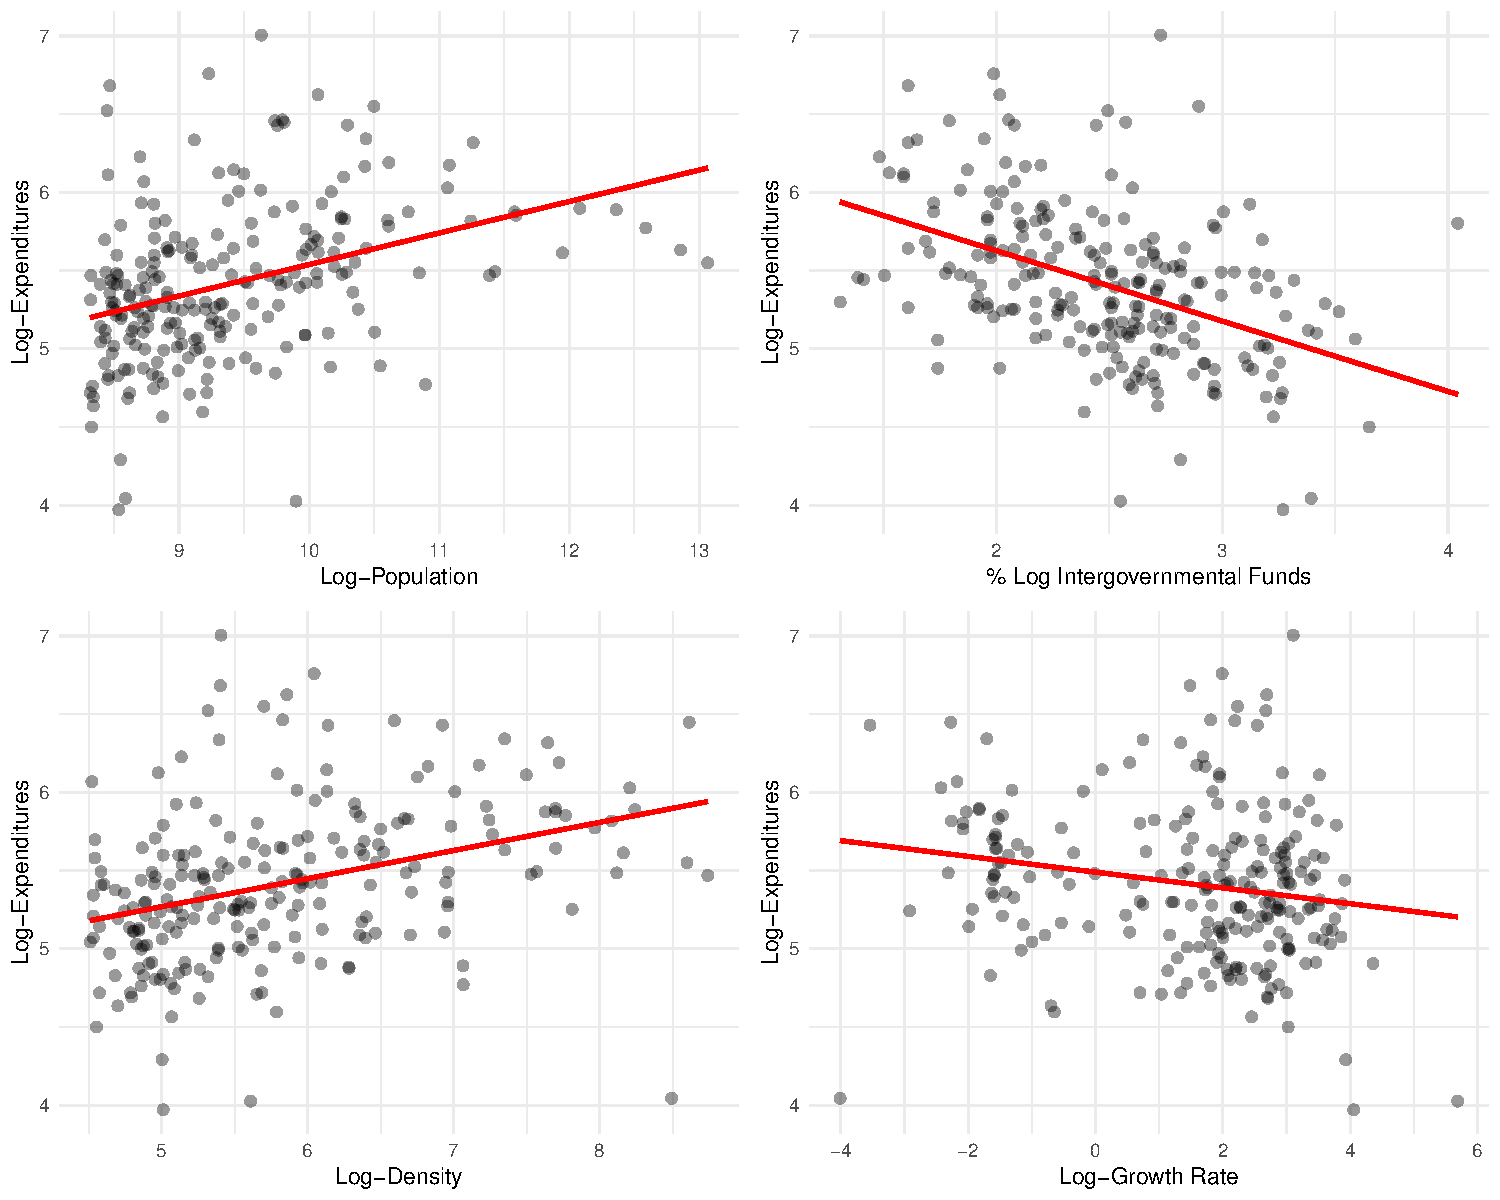
\includegraphics[width=\maxwidth]{figure/unnamed-chunk-12-1} 

\caption{Exploratory plot after log-transformation and subsetted data with linear regression line in red of 1: Log-Expenditures vs Log-Population, 2: Log-Expenditures vs Log-Intergovernmental Funds, 3: Log-Expenditures vs Log-Density, and 4: Log-Expenditures vs Log- Growth Rate.}
\label{sec2-explore}
\end{center} 
\end{figure}


\begin{figure}[h!] 
\begin{center}

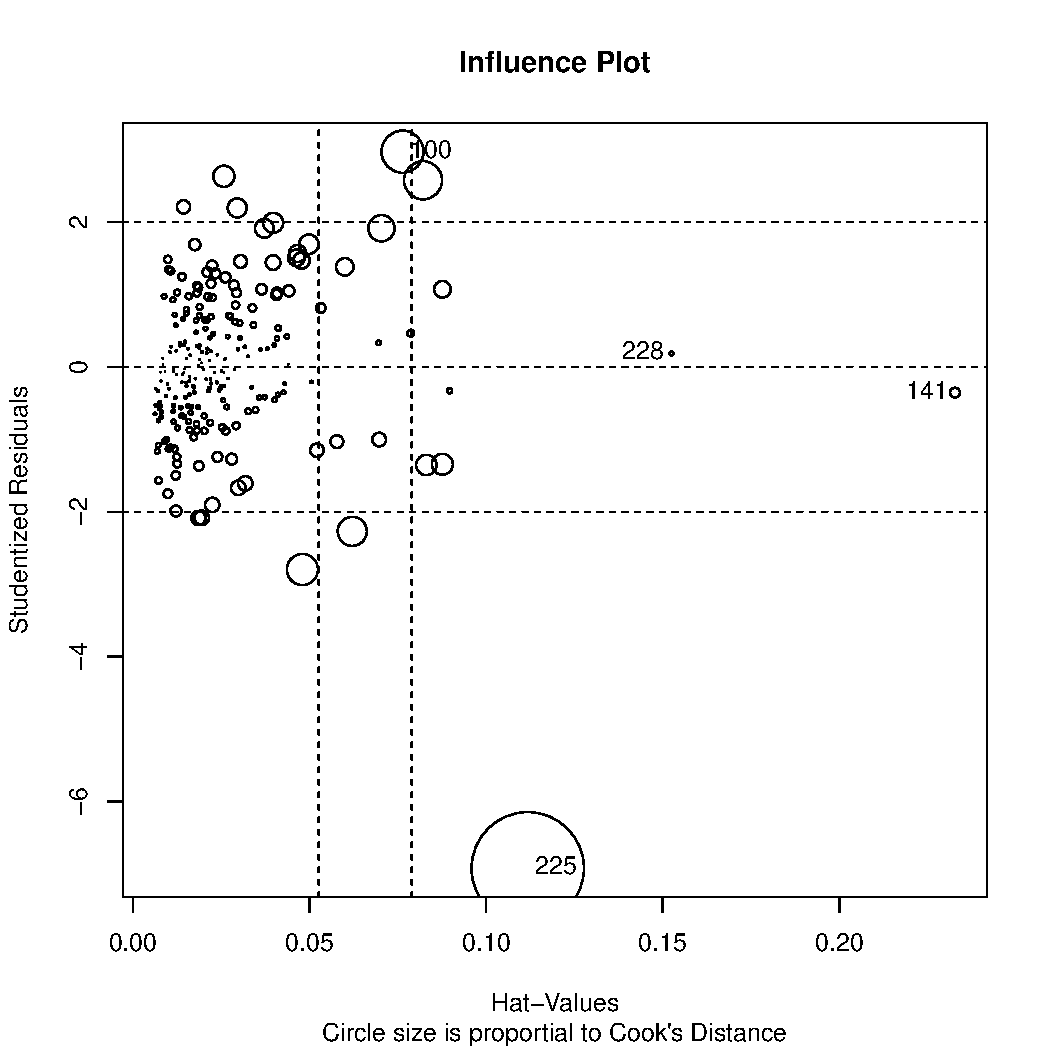
\includegraphics[width=\maxwidth]{figure/unnamed-chunk-13-1} 
       StudRes        Hat       CookD
100  2.9684170 0.07634282 0.117256570
141 -0.3554743 0.23272481 0.006413116
225 -6.9188568 0.11177756 0.829010446
228  0.1863592 0.15245597 0.001045744

\caption{Plot of influential points of studentized residuals vs hat values.}
\label{influential-points}
\end{center} 
\end{figure}

\begin{figure}[h!] 
\begin{center}

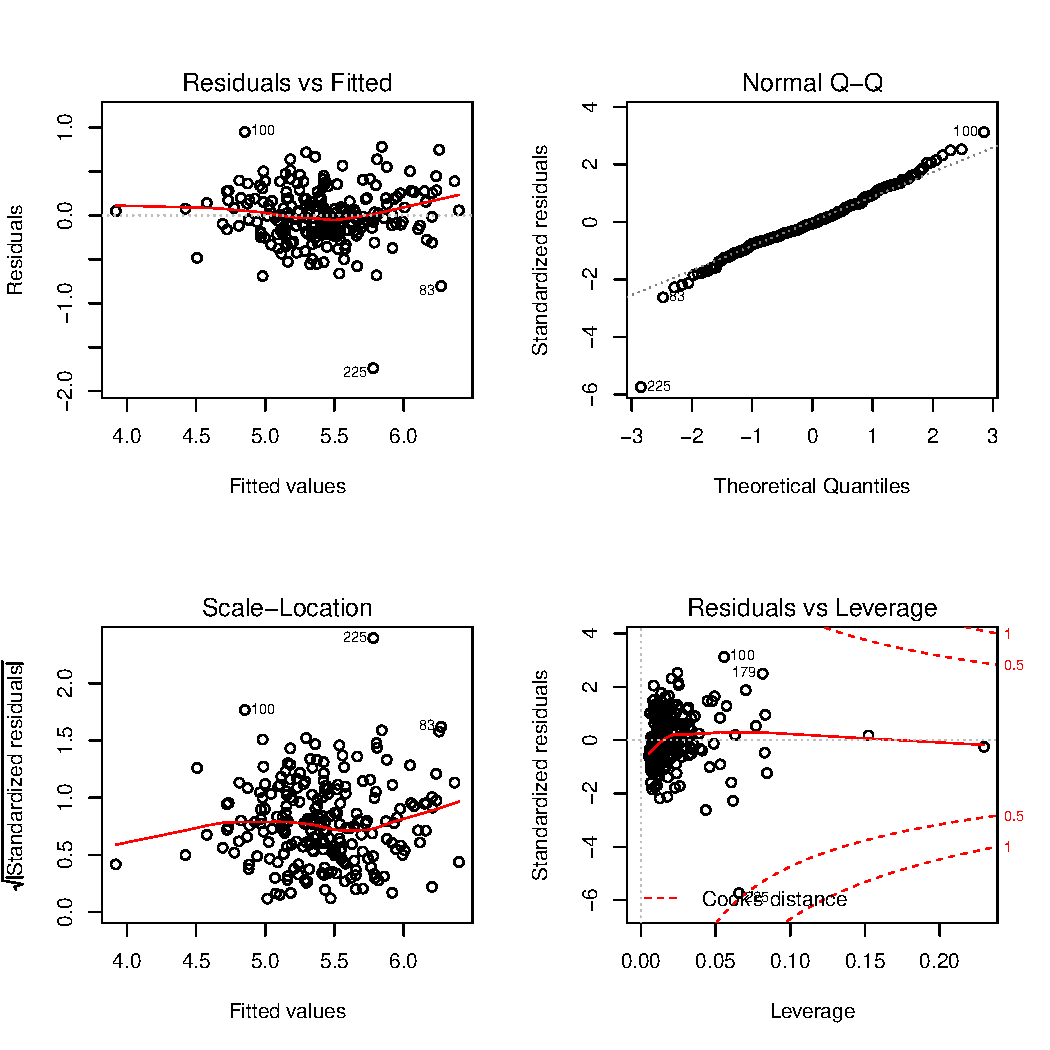
\includegraphics[width=\maxwidth]{figure/unnamed-chunk-14-1} 

\caption{Diagnostics plots}
\label{diag-plot2}
\end{center} 
\end{figure}

\clearpage
\newpage
\noindent \Large{{\bf Appendix C: R Code}}
\lstinputlisting[language=R, caption = Appendix of Code]{R/dar1-codes.R}


\end{document}






